\section{Experimental analysis}\label{sec:method}

\subsection{Research questions and measured scope}
The evaluation distinguishes three evidence sets: a native fixed-center study on eight corpora; a completed Groth16 preprocessing/query study on five of those corpora; and archived sparse-JL ordering and margin experiments. The last set predates the protected-energy construction and is reported as supporting evidence, rather than a measurement of the new protocol. Full-cached native and geometry follow-ups extend the first two sets. We ask:
\begin{description}[leftmargin=1.3cm,style=nextline]
\item[RQ1] How well do the compressed representations preserve fixed-center assignments and original-space clustering cost?
\item[RQ2] What are the measured constraints, timings, memory, and answer errors of the implemented preprocessing/query relation?
\item[RQ3] What do ordering measurements and perturbation/binding controls establish about the proposed protocol?
\item[RQ4] When do the original sparse-JL margin conditions explain stability, and what additional geometry does the residual tail retain?
\item[RQ5] How do small proof shapes, center count, precision and removal of the JL tail affect the measured result?
\end{description}
These questions retain the original evaluation structure. The experiments now include original-data binding and varying subsets, but do not establish a general clustering advantage over PCA, a uniform small-width JL failure bound, or a production-scale DBSCAN proof.

\subsection{Datasets and experimental configurations}
Table~\ref{tab:datasets-a} gives the actual analyzed subsets. Native centers are fitted on a 60\% training split using $k$-means with five initializations, and assignments are audited on the remaining 40\%. The split permutation uses seed $10{,}000+s$, where $s\in\{0,1,2\}$ is the clustering start. The current component grid uses five maps per random setting, $k=5,10$, and widths $m\in\{16,32,64\}$ where rank/budget permits; the geometry follow-up uses ten maps per start/budget. The full-cached native follow-up uses five starts, all 70,000 cached MNIST/Fashion rows, and 10,944 nonzero cached 20 Newsgroups training documents. These are native computations, not whole-corpus proofs.
\begin{table*}[tp]
\caption{Capped native corpora and actual fixed-center proof catalogs.}\label{tab:datasets-a}
\centering\small
\begin{adjustbox}{max width=\textwidth}
\begin{tabular}{@{}lrrrl@{}}
\toprule
Corpus & Native rows & Features $d$ & Audit rows/start & Proof catalog $N$ \\
\midrule
Gaussian-easy & 2,000 & 256 & 800 & -- \\
Gaussian-hard & 2,000 & 512 & 800 & 32 ($k=5,10$) \\
Margin-synthetic & 1,000 & 128 & 400 & -- \\
MNIST & 5,000 & 784 & 2,000 & 16; 64 ($k=5$) \\
Fashion-MNIST & 5,000 & 784 & 2,000 & 16 ($k=5$) \\
Gisette & 3,000 & 5,000 & 1,200 & 8 ($k=5$) \\
Arcene & 100 & 10,000 & 40 & -- \\
20 Newsgroups & 2,913 & 2,000 & 1,166 & 16 ($k=5$) \\
\bottomrule
\end{tabular}
\end{adjustbox}
\par\vspace{3pt}\begin{minipage}{0.98\textwidth}\footnotesize Each capped corpus uses a 60/40 fit/audit split and $k=5,10$ with three starts. Image subsets are sampled by the loader. Text starts with at most 3,000 training documents; zero vectors are removed, leaving 2,913. Gisette uses a 3,000-row cap; Arcene uses 100 cached training rows. Margin-synthetic is used here only for fixed-center and geometry tests, not a DBSCAN proof.\end{minipage}
\end{table*}


The proof control uses Gaussian hard, MNIST, Fashion-MNIST, nonzero 20 Newsgroups, and Gisette. Main catalogs contain the first 8--32 held-out rows at full original feature dimension; a further MNIST catalog contains 64. Each method receives the same committed integer points and centers within a matched catalog. PCA is randomized PCA fitted on training data. Protected directions are derived from the public center differences. Width is 16 for PCA and protected+energy+JL; the no-JL control stores $h+1\leq k$ values. Energy has squared-scale units and a wider range, so equal column counts do not imply equal storage bits. Exact affine and cached-answer controls reproduce quantized Full for the fixed task. In the tables, CommitJL-16 denotes head+energy+JL, while head+energy is the no-tail control.

The main campaign completes 30 method/catalog bundles and 480 Stage-1 row proofs. The follow-up adds 32 actual pair-distance configurations and 30 full-cached native jobs. All 96 completion jobs finish, including 24 matched proof controls, six larger-catalog jobs and 66 native corpus/$k$/start cells. Its 7,776 rows include maps, precision settings and ablations, not independent datasets. Query batches use three measured repetitions after one warmup, and genuinely distinct subsets where possible. Twenty-four unique native configurations are excluded for PCA fitting rank or insufficient protected-head budget; repeated map IDs do not count as new exclusions. Other large Full proof shapes remain unmeasured, rather than extrapolated.

MNIST/Fashion are loaded through OpenML, Gisette/Arcene through the UCI training files, and text through the recorded training loader \cite{lecun1998,fashion2017,gisette2004,arcene2004,news20data}. The text vocabulary/TF--IDF weights are fitted before the center/PCA split; headers, footers and quotes are removed and English stop words filtered. Input scaling uses the loaded corpus maximum. The image source partitions are pooled by the loader and then resplit. These choices define a fixed-corpus audit, not an unseen-data predictive-learning benchmark. Public class labels do not enter fidelity metrics.

\subsection{Metrics and statistical interpretation}
Let $a_i^{\rm full}$ be the original-space nearest-center assignment and $a_i^M$ the assignment from representation $M$, using first-index ties. The original-space assignment-cost ratio is
\begin{equation}
r_\Phi(M)=\frac{\sum_i\|x_i-c_{a_i^M}\|^2}{\sum_i\|x_i-c_{a_i^{\rm full}}\|^2}.
\end{equation}
Assignment agreement and adjusted Rand index (ARI) compare these two outputs, not external class labels. Separately, the signed claimed-cost error is
\begin{equation}
e_\Psi=\frac{\widehat\Psi/D_M}{\sum_i\|x_i-c_{a_i^{\rm full}}\|^2}-1,
\end{equation}
where $D_M=S^2T^4$ for the rounded head/PCA representations and $D_M=S^2$ for Full, affine and cached exact answers. The reference precision is stated explicitly; integer Full can disagree with floating Full near boundaries. A small $r_\Phi$ does not imply a small $e_\Psi$: assignments can remain stable while discarded directions contribute substantial original-space energy.

The archived native fidelity qualification requires the lower 95\% ARI bound to be at least 0.8 and the upper 95\% $r_\Phi$ bound to be at most 1.1. We recompute pointwise intervals using 2,000 crossed-bootstrap resamples of the map and start axes. In that archived cohort PCA has one map per start and randomized representations have ten. Current component maps are first averaged within a fitted start, then corpus/$k$ cells are weighted equally. There are only three starts, and the intervals are conditional on the fixed corpora. These are exploratory qualification checks using the manuscript's stated thresholds, not a prospective registration or a multiplicity-adjusted superiority test. Repeated proofs measure machine variation on a fixed instance, not geometric generalization \cite{kalibera2013effect}.

Current pairwise geometry is summarized separately by sampled mean absolute relative squared-distance error and recall@10. Methods are compared on matched corpus/$k$/start cells at each width; the width-trend plot uses the same 42 cells at every width. Energy is excluded from Euclidean coordinates. Archived distortion quantiles retain their older scope. For proof performance, compile, circuit-specific setup, witness generation, prove, and verify times remain separate. Reported RSS is a sampled peak of the CLI process tree including setup; the Python orchestration process is outside that measurement. The current process guard limits child RSS to 5.3\,GiB, reserves 768\,MiB of host memory, and sets a finite 2,400\,s phase deadline. Reconstructed workloads add measured components rather than claiming observed elapsed time or a break-even threshold.

\subsection{Results}\label{sec:results}
\subsubsection{RQ1: fixed-center fidelity}
In the archived qualification cohort, both protected variants satisfy the stated confidence-bound rule in all 16 dataset/$k$ cells at $m=16$, compared with 12 for PCA and none for sparse JL (Table~\ref{tab:eligibility}). Those older intervals are retained as supporting evidence and are not pooled with the new fixed-point cohort. Width 16 remains the smallest tested width, not a mathematical minimum.
\begin{table*}[tp]
\caption{Confidence-bound fidelity qualification across all 16 dataset/$k$ cells.}\label{tab:eligibility}
\centering\scriptsize
\begin{adjustbox}{max width=\textwidth}
\begin{tabular}{@{}lll@{}}
\toprule
Method & Pass at $m=16$ & Pass at any tested width \\
\midrule
PCA & 12/16 & 15/16 \\
Sparse JL & 0/16 & 6/16 \\
Protected + JL & 16/16 & 16/16 \\
Protected integer & 16/16 & 16/16 \\
\bottomrule
\end{tabular}
\end{adjustbox}
\par\smallskip
\begin{minipage}{\textwidth}\scriptsize Pass requires ARI lower bound $\geq0.8$ and $r_\Phi$ upper bound $\leq1.1$. $m=16$ is the smallest tested width, not a proven minimum. Widths above the training rank are unavailable for PCA.\end{minipage}
\end{table*}


Table~\ref{tab:fidelity-a} updates the detailed comparison to all eight capped corpora and both $k=5,10$ using the completed fixed-point/component study. Protected assignment is exact in real arithmetic because the head spans the fixed public center differences. It is therefore a task-specific identity rather than evidence of an unusually favorable random projection. Integer discrepancies reflect finite precision. Exact fixed-center assignment does not imply accurate pairwise geometry or accurate original-space cost recovery from a plain tail norm.
\begin{table*}[tp]
\caption{Fixed-center fidelity on eight capped corpora at storage budget 16.}\label{tab:fidelity-a}
\centering\small
\begin{adjustbox}{max width=\textwidth}
\begin{tabular}{@{}lrrrrrr@{}}
\toprule
Corpus & $k$ & Sparse ARI & PCA ARI & Head/E ARI & PCA agree. (\%) & Head/E agree. (\%) \\
\midrule
Gaussian-easy & 5 & 0.62947 & 1.00000 & 1.00000 & 100.000 & 100.000 \\
Gaussian-easy & 10 & 0.87790 & 1.00000 & 1.00000 & 100.000 & 100.000 \\
Gaussian-hard & 5 & 0.11602 & 0.99365 & 1.00000 & 99.792 & 100.000 \\
Gaussian-hard & 10 & 0.15151 & 0.99359 & 1.00000 & 99.000 & 100.000 \\
Margin-synthetic & 5 & 0.18329 & 0.62386 & 0.99640 & 89.833 & 99.917 \\
Margin-synthetic & 10 & 0.21543 & 0.49844 & 1.00000 & 79.167 & 100.000 \\
MNIST & 5 & 0.36872 & 0.98165 & 0.99960 & 99.183 & 99.983 \\
MNIST & 10 & 0.36090 & 0.92547 & 0.99964 & 96.567 & 99.983 \\
Fashion-MNIST & 5 & 0.66488 & 0.99484 & 1.00000 & 99.783 & 100.000 \\
Fashion-MNIST & 10 & 0.64867 & 0.98679 & 0.99958 & 99.317 & 99.983 \\
Gisette & 5 & 0.14792 & 0.96671 & 0.99917 & 98.694 & 99.972 \\
Gisette & 10 & 0.12200 & 0.92786 & 1.00000 & 96.861 & 100.000 \\
Arcene & 5 & 0.85164 & 1.00000 & 1.00000 & 100.000 & 100.000 \\
Arcene & 10 & 0.67673 & 0.95751 & 1.00000 & 97.500 & 100.000 \\
20 Newsgroups & 5 & 0.01789 & 0.82891 & 1.00000 & 93.511 & 100.000 \\
20 Newsgroups & 10 & 0.00868 & 0.61244 & 1.00000 & 78.988 & 100.000 \\
\bottomrule
\end{tabular}
\end{adjustbox}
\par\vspace{3pt}\begin{minipage}{0.98\textwidth}\footnotesize Reference: quantized Full. Means over three fitted starts; sparse maps are averaged within a start before aggregation. Head/E and CommitJL have identical fixed-center outputs. Sparse JL uses one signed bucket per input column. ARI measures assignment fidelity, not agreement with class labels.\end{minipage}
\end{table*}

\begin{table*}[tp]
\caption{Native fidelity on all cached image rows and nonzero cached text-training rows.}\label{tab:full-accuracy}
\centering\small
\begin{adjustbox}{max width=\textwidth}
\begin{tabular}{@{}lrrrrrr@{}}
\toprule
Corpus & $k$ & PCA ARI$_Q$ & Ours ARI$_Q$ & PCA agree.$_Q$ (\%) & Ours agree.$_Q$ (\%) & Ours agree.$_F$ (\%) \\
\midrule
MNIST & 5 & 0.97712 & 0.99974 & 99.072 & 99.990 & 99.989 \\
MNIST & 10 & 0.93466 & 0.99975 & 96.956 & 99.989 & 99.989 \\
Fashion-MNIST & 5 & 0.99601 & 0.99987 & 99.831 & 99.994 & 99.995 \\
Fashion-MNIST & 10 & 0.98809 & 0.99988 & 99.416 & 99.994 & 99.994 \\
20 Newsgroups & 5 & 0.88163 & 0.99920 & 95.724 & 99.968 & 99.712 \\
20 Newsgroups & 10 & 0.82280 & 0.99945 & 92.289 & 99.973 & 99.785 \\
\bottomrule
\end{tabular}
\end{adjustbox}
\par\vspace{3pt}\begin{minipage}{0.98\textwidth}\footnotesize Subscripts $Q$ and $F$ denote quantized-Full and floating-Full references. Five fitted starts per corpus/$k$; 60/40 fitting/audit split. MNIST and Fashion-MNIST: 70,000 rows each (28,000 audit rows). Text: 10,944 nonzero training documents, 2,000 TF--IDF features (4,378 audit rows). These are native runs, not whole-corpus proofs. Ours denotes both head/energy variants.\end{minipage}
\end{table*}


On full cached data, head+energy and CommitJL-16 have identical fixed-center outputs: mean ARI 0.999647 and agreement 99.9845\% against quantized Full, versus PCA-16's 0.933384 and 97.2146\%. Against floating Full the protected figures are ARI 0.997434 and agreement 99.9108\%; quantized Full itself gives 0.997491 and 99.9129\%. This reference distinction prevents input-rounding error from being mistaken for a loss caused solely by compression. Five-start variation and unrounded per-cell exports are retained in the artifact.
\begin{figure*}[tp]
\centering
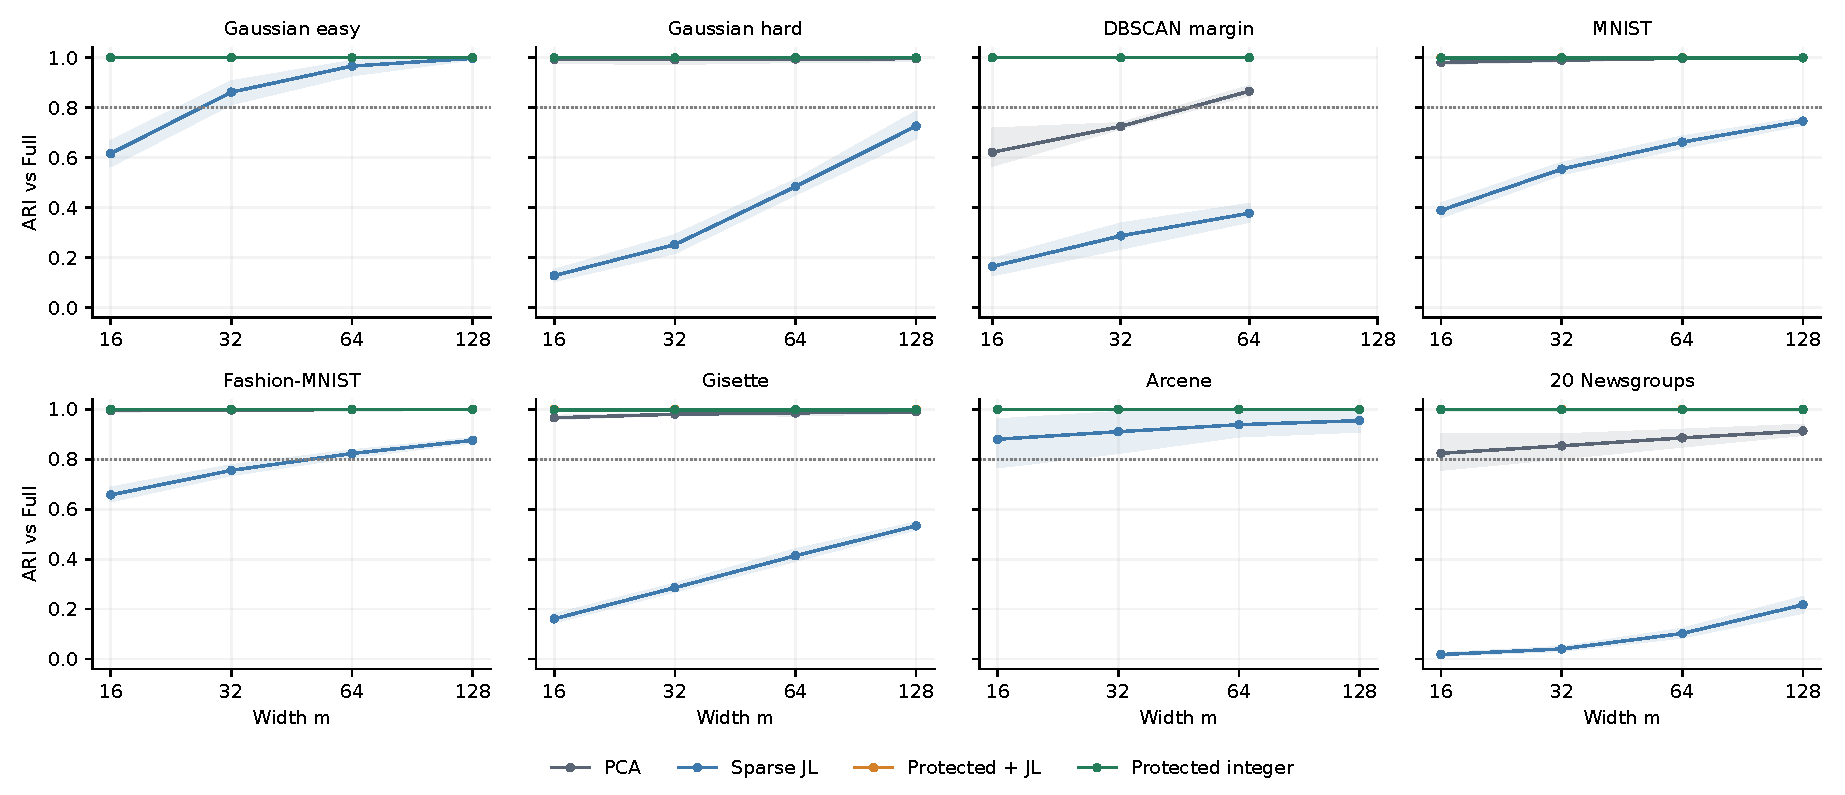
\includegraphics[width=\textwidth]{paper_results/figures/fidelity.pdf}
\caption{Native ARI versus width at $k=5$. Bands are pointwise crossed-bootstrap intervals. PCA curves stop where the training-rank restriction excludes a width; no missing cells are interpolated. The horizontal line is the ARI threshold, and cost qualification must also hold.}
\label{fig:fidelity-results}
\end{figure*}
Figure~\ref{fig:fidelity-results} retains the archived native qualification study; it is separate from the new rounded-input full-cached comparison. It shows why there is no single dataset-independent width ranking. In particular, low-margin text and the DBSCAN-margin corpus remain difficult for PCA and unprotected sparse JL. The protected identity addresses the fixed centers used here; it does not establish that the same representation supports arbitrary new centers or newly fitted clusters.

\subsubsection{RQ2: measured proof cost and numerical accuracy}
For eight-point batches, Table~\ref{tab:zkperf-a} updates the original query-cost comparison to actual proofs in the completed Poseidon2 cohort. On Gaussian-hard, CommitJL-16 takes 0.882\,s versus 1.037\,s for PCA at $k=5$, and 1.051 versus 1.101\,s at $k=10$. Each other displayed protected query is also faster than its PCA-16 comparator, while the affine control is frequently cheaper. These are observed timings, not confidence-bounded universal speedups. Setup is circuit-specific and must be counted when centers or shape change.
\begin{table*}[tp]
\caption{Actual eight-record fixed-center query proving time (seconds).}\label{tab:zkperf-a}
\centering\small
\begin{adjustbox}{max width=\textwidth}
\begin{tabular}{@{}lrrrrrr@{}}
\toprule
Corpus & $k$ & Full & PCA-16 & Head + energy & CommitJL-16 & Exact affine \\
\midrule
Gaussian-hard & 5 & 11.723 & 1.037 & 0.890 & 0.882 & 0.594 \\
Gaussian-hard & 10 & 11.377 & 1.101 & 1.007 & 1.051 & 0.935 \\
MNIST & 5 & 18.519$^{\dagger}$ & 1.057 & 0.831 & 0.829 & 0.596 \\
Fashion-MNIST & 5 & 17.869$^{\dagger}$ & 1.045 & 0.822 & 0.846 & 0.592 \\
20 Newsgroups & 5 & -- & 1.021 & 0.840 & 0.841 & 0.600 \\
Gisette & 5 & -- & 0.967 & 0.588 & 0.594 & 0.596 \\
\bottomrule
\end{tabular}
\end{adjustbox}
\par\vspace{3pt}\begin{minipage}{0.98\textwidth}\footnotesize Compilation, setup and Stage 1 excluded. Three measured repetitions after one warmup, summarized across distinct subsets. Main $b=8$ runs have eight subsets when $N>8$; Gisette has one full-catalog subset. $^{\dagger}$Additional Full controls use two subsets at a 1.5M-constraint ceiling. Dashes are unmeasured resource-budget exclusions, not observed out-of-memory failures.\end{minipage}
\end{table*}

\begin{table*}[tp]
\caption{Original-space diagnostics for matched actual-proof configurations.}\label{tab:cost-error}
\centering\small
\begin{adjustbox}{max width=\textwidth}
\begin{tabular}{@{}lrrrr@{}}
\toprule
Method & Configurations & Mean agree. (\%) & Median signed cost error (\%) & Max abs. cost error (\%) \\
\midrule
PCA-16 & 13 & 96.995 & -93.021784 & 97.044456 \\
Head + energy & 13 & 100.000 & 0.000558 & 0.007886 \\
CommitJL-16 & 13 & 100.000 & 0.000558 & 0.007886 \\
Exact affine & 13 & 100.000 & -0.000097 & 0.007590 \\
\bottomrule
\end{tabular}
\end{adjustbox}
\par\vspace{3pt}\begin{minipage}{0.98\textwidth}\footnotesize Floating Full reference; 13 matched catalog/query-size configurations per method with batch size at least eight. Agreement is averaged within each configuration before aggregation. The signed-error column is the median of per-configuration signed medians; the maximum uses every recorded subset. It is not a mean absolute error. One-record ARI is uninformative. Assignment diagnostics are private harness metadata.\end{minipage}
\end{table*}


On the 13 matched actual-proof configurations with at least eight queried records, head+energy, CommitJL and affine have observed agreement 100\% with floating Full, versus PCA's mean 96.995\%. These small nested subsets are not independent point samples or replacements for the larger native study. PCA proves its projected cost correctly; its original-space proxy error does not invalidate the proof. The signed-median and worst-error summaries in Table~\ref{tab:cost-error} are labeled separately from mean absolute cost error.

Full-dimensional batch-eight image controls now complete at 1,311,683 constraints/18.519\,s for MNIST and 1,311,719/17.869\,s for Fashion-MNIST, with peak RSS below 2.4\,GB and independent public verification. Table~\ref{tab:earlier-full} reports them alongside matched Gaussian Full controls. Other large Full shapes are unmeasured, not observed out-of-memory failures or filled estimates. In the 84 completed main query configurations, proofs are 196 bytes and the median of configuration-level verification medians is 4.086\,ms (range 2.696--6.196\,ms); registering a compressed catalog additionally requires all Stage-1 verifications.
\begin{table*}[tp]
\caption{Full-dimensional controls in the same completed Poseidon2 cohort.}\label{tab:earlier-full}
\centering\small
\begin{adjustbox}{max width=\textwidth}
\begin{tabular}{@{}lrrrrr@{}}
\toprule
Corpus & $k$ & Catalog $N$ & Batch $b$ & Constraints & Proving (s) \\
\midrule
Gaussian-hard & 5 & 32 & 8 & 866,346 & 11.723 \\
Gaussian-hard & 10 & 32 & 8 & 869,866 & 11.377 \\
MNIST & 5 & 16 & 8 & 1,311,683 & 18.519 \\
Fashion-MNIST & 5 & 16 & 8 & 1,311,719 & 17.869 \\
\bottomrule
\end{tabular}
\end{adjustbox}
\par\vspace{3pt}\begin{minipage}{0.98\textwidth}\footnotesize All rows are actual independently verified proofs, not projected constraint estimates. Image controls use two distinct subsets at a 1.5M ceiling; Gaussian controls use eight. Other larger Full shapes remain unmeasured. A preflight exclusion is not an observed out-of-memory failure.\end{minipage}
\end{table*}


On the larger 64-record MNIST catalog at $k=5$, the whole-catalog query uses 306,274 constraints and 5.087\,s for CommitJL, versus 472,429 and 6.303\,s for PCA-16. Cached exact answers use 197,147 and 3.442\,s. Affine has fewer constraints than CommitJL, although time ordering varies. A whole-catalog query has only one possible subset; repeating it measures machine variation, not distinct workloads.
\begin{table*}[tp]
\caption{Preprocessing and reconstructed fresh-workload cost, MNIST $N=64$, $k=5$.}\label{tab:preprocessing}
\centering\small
\begin{adjustbox}{max width=\textwidth}
\begin{tabular}{@{}lrrrrr@{}}
\toprule
Method & \shortstack{Stage-1\\constraints/row} & \shortstack{Median row\\proof (s)} & \shortstack{All row\\proofs (s)} & \shortstack{Stage-1\\compile/setup (s)} & \shortstack{Four-query\\workload (s)} \\
\midrule
PCA-16 & 170,744 & 3.087 & 197.961 & 29.011 & 279.123 \\
Head + energy & 168,901 & 3.067 & 196.990 & 28.372 & 264.617 \\
CommitJL-16 & 174,208 & 3.083 & 198.221 & 29.350 & 268.383 \\
Exact affine & 168,815 & 3.058 & 195.780 & 29.559 & 268.288 \\
Cached exact & 168,446 & 3.014 & 194.488 & 27.153 & 246.660 \\
\bottomrule
\end{tabular}
\end{adjustbox}
\par\vspace{3pt}\begin{minipage}{0.98\textwidth}\footnotesize The workload uses four genuinely distinct 32-record subsets. It adds native Go preparation, all 64 Stage-1 witness/proof costs, Stage-1 and query compilation/setup, and one witness/proof per subset. Public-model fitting, verification, warmups and I/O are excluded. These sums reconstruct measured components; they are not observed elapsed times or an empirical break-even threshold.\end{minipage}
\end{table*}

\begin{figure*}[tp]
\centering
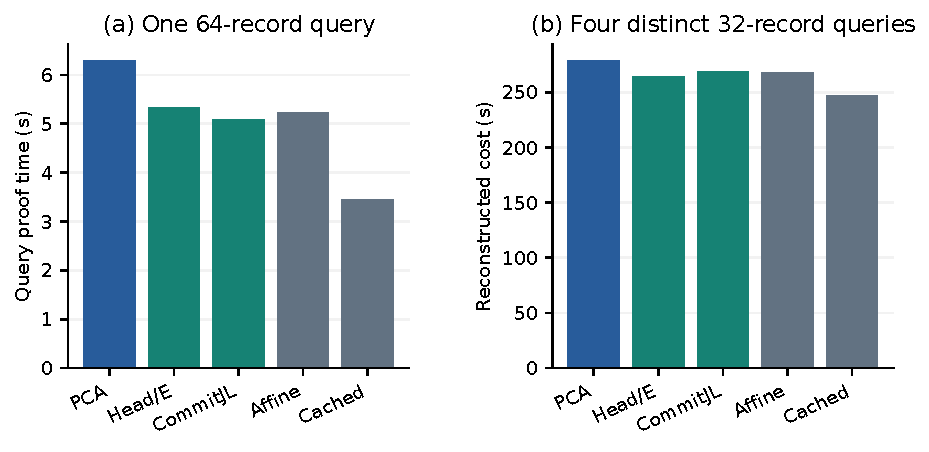
\includegraphics[width=0.94\textwidth]{paper_results/bound_revision/figures/proof_costs.pdf}
\caption{Query-only cost and preprocessing-inclusive reconstructed workload on the 64-record MNIST catalog. The latter uses four genuinely different 32-record subsets and is a sum of measured components, not elapsed wall time.}
\label{fig:measured-stages}
\end{figure*}
Figure~\ref{fig:measured-stages} separates the measured costs. Stage 1 is now included: CommitJL's 64 row proofs sum to 198.221\,s, plus 29.350\,s of preprocessing compile/setup. The reconstructed fresh four-query workload totals 268.383\,s for CommitJL, 279.123\,s for PCA, 264.617\,s for head+energy, 268.288\,s for affine and 246.660\,s for cached answers. It includes Go preparation, all preprocessing witness/proof costs, both compile/setup shapes and one proof per subset; public-model fitting, verification, warmups and I/O are excluded. The advantage over PCA is 3.85\%, smaller than a query-only ratio. Full needs no Stage 1 and is cheaper for the tested small one-record workload. No measured break-even threshold is established.

\subsubsection{RQ3: ordering and adversarial controls}
The archived host-side ordering study measures an additional 25.40--31.58\,ms for postcommit ordering over a prepublished transform, depending on the local source (Table~\ref{tab:ordering-a}). Each source has ten task clusters and 100 paired observations; task-bootstrap intervals exclude zero. The beacon and commit--reveal cases are local simulations, not deployed distributed entropy services. These timings do not include an original-data preprocessing proof, nor do they measure the marginal cost of sampling the unused tail in the energy circuit.
\begin{table*}[!htbp]
\caption{Archived host-side ordering study (6--7 October), not a Stage-1 proof benchmark.}\label{tab:ordering-a}
\centering\scriptsize
\begin{adjustbox}{max width=\textwidth}
\begin{tabular}{@{}lllllll@{}}
\toprule
Local source & Tasks & Pairs & Prepublished (s) & Postcommit (s) & $\Delta$ (ms) & 95\% CI (ms) \\
\midrule
beacon & 10 & 100 & 0.5226 & 0.5480 & 25.39 & [16.42, 32.47] \\
commit\_reveal & 10 & 100 & 0.5199 & 0.5487 & 28.89 & [19.69, 37.78] \\
nonce & 10 & 100 & 0.5202 & 0.5517 & 31.58 & [22.60, 39.72] \\
\bottomrule
\end{tabular}
\end{adjustbox}
\par\smallskip
\begin{minipage}{\textwidth}\scriptsize Intervals resample task means. Beacon and commit--reveal sources are local simulations; network and distributed-service costs are absent. These data characterize the earlier sparse protocol and do not measure the complete protected preprocessing stage.\end{minipage}
\end{table*}

\begin{table*}[!htbp]
\caption{Earlier native perturbation controls; no forged end-to-end proofs are generated.}\label{tab:attack-controls}
\centering\scriptsize
\begin{adjustbox}{max width=\textwidth}
\begin{tabular}{@{}lllll@{}}
\toprule
Projection/order & True inflation & Claim inflation & Flip fraction & Honest error \\
\midrule
pca\_public & 11.000 & 1.000 & 0.9762 & 0.0273 \\
protected\_commit & 11.000 & 11.010 & 0.0000 & 0.0000 \\
protected\_prepublished & 11.000 & 1.000 & 0.0000 & 0.0000 \\
sparse\_commit & 10.988 & 11.138 & 0.6082 & 0.3715 \\
sparse\_prepublished & 10.988 & 1.000 & 0.8578 & 0.3713 \\
\bottomrule
\end{tabular}
\end{adjustbox}
\par\smallskip
\begin{minipage}{\textwidth}\scriptsize Protected rows test the linear head+tail representation, not head+energy. Fresh-map rows use one independently guessed-map strategy. Flip and honest-error fractions concern different point sets and cannot be subtracted to isolate attack advantage. The unverified internal Pisot surrogate is excluded from comparisons with published methods.\end{minipage}
\end{table*}


Table~\ref{tab:attack-controls} reproduces the earlier native perturbation study. For known linear projections, constructed kernel perturbations increase the original cost by roughly $11\times$ while leaving projected cost unchanged. However, both prepublished and postcommit protected variants have zero assignment flips in this study. The protected attack implementation uses the linear head+tail sketch, not the energy representation; the fresh-map attacker guesses one independent map rather than optimizing over all admissible strategies. The unverified internal Pisot surrogate is excluded from claims about the published comparator. These controls neither establish an attack on that published construction nor prove universal security of CommitJL.

Earlier native controls on all ten proof-dataset/$k$ combinations recover the original cost inflation using head+energy without any JL tail, even when the linear projection is known in advance. This follows from the exact energy identity. It does not remove the need to prove that the stored energy is honestly derived. In an archived query-only actual-proof control, setting one stored energy to zero and recomputing its compressed commitment changes the claimed integer cost from 8,338,008,232 to 87,484,126 and still yields a valid Stage-2 proof. This is an expected acceptance under a different public root, not a collision or a forgery under the original root. An original-data binding proof must reject the assertion that these altered statistics represent the same original committed record. The completed implementation now supplies that missing obligation through all-index Stage-1 derivation proofs; the archived changed-root acceptance is not a bypass of those proofs.

The new original-data binding checks complement these archived controls. Fresh checking passes 22,645 consistency/proof checks, including 1,109 saved-proof verifications across 32 public bundles without private arrays or assignment logs. Missing preprocessing indices, changed roots/keys and altered statistics are covered by relation tests. This does not establish model training, host challenge ordering or a formal security audit. In particular, the 64-row catalog reuses an earlier approved matrix; its performance does not demonstrate fresh geometric independence for that new root.

\subsubsection{RQ4: margin interpretation and its limits}
Defined conditional-violation rates in the selected archived sparse-JL cells are zero (Table~\ref{tab:cert-a}); undefined aggregates are retained as undefined rather than replaced by zero. Qualified coverage varies strongly by dataset. Qualification checks both the original margin and the realized embedding event, so this is a post hoc validation of the sufficient-condition logic, not a verifier-side certificate available from the margin alone. Conditional zero violations do not imply that every assignment or neighborhood is preserved.
\begin{table*}[!htbp]
\caption{Archived sparse-JL margin checks at $m=128,q=2$ (assignment: $k=5$).}\label{tab:cert-a}
\centering\scriptsize
\begin{adjustbox}{max width=\textwidth}
\begin{tabular}{@{}llllllll@{}}
\toprule
Query & Dataset & $n$ & Draws & Qualified coverage & Conditional violations & Uncert. stability & ARI \\
\midrule
Assignment & 20 Newsgroups & 3000 & 50 & 0.0122 & undefined & 0.6216 & 0.2660 \\
Assignment & Arcene & 100 & 50 & 0.3344 & 0.0000 & 0.9937 & 0.9906 \\
Assignment & DBSCAN margin & 1000 & 50 & 0.1139 & undefined & 0.8851 & 0.6673 \\
Assignment & Fashion-MNIST & 5000 & 50 & 0.2374 & 0.0000 & 0.9306 & 0.8761 \\
Assignment & Gaussian easy & 2000 & 50 & 0.3515 & 0.0000 & 1.0000 & 1.0000 \\
Assignment & Gaussian hard & 2000 & 50 & 0.3334 & 0.0000 & 1.0000 & 1.0000 \\
Assignment & Gisette & 3000 & 50 & 0.0046 & 0.0000 & 0.8075 & 0.5749 \\
Assignment & MNIST & 5000 & 50 & 0.1967 & 0.0000 & 0.8758 & 0.7644 \\
DBSCAN & 20 Newsgroups & 1000 & 10 & 0.7279 & 0.0000 & 0.8650 & 0.0148 \\
DBSCAN & Arcene & 100 & 10 & 0.7425 & 0.0000 & 0.9278 & 0.8527 \\
DBSCAN & DBSCAN margin & 1000 & 10 & 0.7694 & 0.0000 & 0.9994 & 1.0000 \\
DBSCAN & Fashion-MNIST & 1000 & 10 & 0.7409 & 0.0000 & 0.9871 & 0.7753 \\
DBSCAN & Gaussian easy & 1000 & 10 & 0.7144 & 0.0000 & 0.8879 & 0.7413 \\
DBSCAN & Gaussian hard & 1000 & 10 & 0.6893 & 0.0000 & 0.9013 & 0.7234 \\
DBSCAN & Gisette & 1000 & 10 & 0.6494 & 0.0000 & 0.8438 & 0.1699 \\
DBSCAN & MNIST & 1000 & 10 & 0.7543 & 0.0000 & 0.9813 & 0.5496 \\
\bottomrule
\end{tabular}
\end{adjustbox}
\par\smallskip
\begin{minipage}{\textwidth}\scriptsize Fractions are means over the recorded draws, not pooled counts. Qualification conditions on the realized embedding checks and margin; zero conditional violations do not imply unconditional stability. Assignment uses 50 map/start observations; DBSCAN uses 10 maps. This supporting study predates the protected-energy circuit.\end{minipage}
\end{table*}


In particular, the archived DBSCAN grid has zero exact-neighborhood-graph preservation across all 720 draws (72 cells with ten maps each), despite substantial pair-level qualified coverage. Exact DBSCAN graph preservation and pair-level conditional soundness are different endpoints. No DBSCAN circuit or protected-energy DBSCAN result is claimed. The new head-based exact assignment property is specific to the fixed center span and does not replace the pairwise embedding requirements of the neighborhood theorem.

The completed residual-geometry follow-up now measures the tail separately. At budget 16, matched mean absolute squared-distance error is 28.203\% for CommitJL versus 62.406\% for PCA, but recall@10 is lower, 24.500\% versus 42.312\%. At 64, matched error is 11.482\% versus 50.856\%, while recall remains lower, 33.976\% versus 50.253\%. Each budget compares the same corpus/$k$/start cells across methods; Arcene is excluded from both at 64 because PCA exceeds training rank. Energy is excluded from Euclidean coordinates, leaving 15 geometry coordinates at a 16-statistic budget. Native maps are reproducible evaluation maps rather than the exact challenged proof matrices.
\begin{table*}[tp]
\caption{Matched native geometry quality at equal total statistic budgets.}\label{tab:geometry}
\centering\small
\begin{adjustbox}{max width=\textwidth}
\begin{tabular}{@{}lrrrr@{}}
\toprule
Budget $m$ & Method & Matched cells & Mean abs. squared-distance error (\%) & Recall@10 (\%) \\
\midrule
16 & PCA & 48 & 62.406 & 42.312 \\
16 & CommitJL & 48 & 28.203 & 24.500 \\
32 & PCA & 48 & 55.852 & 48.820 \\
32 & CommitJL & 48 & 16.447 & 33.111 \\
64 & PCA & 42 & 50.856 & 50.253 \\
64 & CommitJL & 42 & 11.482 & 33.976 \\
\bottomrule
\end{tabular}
\end{adjustbox}
\par\vspace{3pt}\begin{minipage}{0.98\textwidth}\footnotesize Eight capped corpora, $k=5,10$, three starts, ten maps per start/budget for the random tail. Cells are matched separately at each budget. Arcene is excluded from both methods at 64 because PCA exceeds the fit rank. Pairs are sampled; nearest neighbors use up to 128 held-out queries. Energy is excluded from Euclidean coordinates; CommitJL has $m-1$ such coordinates and one energy statistic. Native maps differ from the post-commit maps in proof bundles.\end{minipage}
\end{table*}

\begin{table*}[tp]
\caption{Actual authenticated pair-distance proofs, storage budget 16.}\label{tab:pair-proofs}
\centering\small
\begin{adjustbox}{max width=\textwidth}
\begin{tabular}{@{}lrrrrr@{}}
\toprule
Corpus & $k$ & PCA constraints & Ours constraints & PCA prove (s) & Ours prove (s) \\
\midrule
Gaussian-hard & 5 & 13158 & 17831 & 0.333 & 0.453 \\
Gaussian-hard & 10 & 13158 & 17823 & 0.312 & 0.482 \\
MNIST & 5 & 12407 & 16330 & 0.333 & 0.344 \\
20 Newsgroups & 5 & 12407 & 16370 & 0.300 & 0.349 \\
\bottomrule
\end{tabular}
\end{adjustbox}
\par\vspace{3pt}\begin{minipage}{0.98\textwidth}\footnotesize Eight distinct pairs, three repetitions after warmup. All saved proofs verify. The circuit proves distance in the stored embedding, not its accuracy relative to the original space. Ours authenticates head and tail through separate roots; PCA uses one representation root. The complete 32-configuration study also includes budgets 32/64 and Full/head controls.\end{minipage}
\end{table*}


All 32 authenticated pair-proof configurations verify, but head/tail pair proofs are generally slower than PCA because they authenticate separate roots. For Gaussian-hard, $k=5$, budget 16, the times are 0.453 versus 0.333\,s. The proof certifies the stored embedding distance; its original-space quality is measured separately. Thus the tail offers lower distance-magnitude distortion here, not a universal neighborhood or proof-speed advantage.

\subsubsection{RQ5: small-shape scaling and tail ablation}
Table~\ref{tab:sensitivity-a} reports measured constraints and proving time as the requested subset grows within the 64-record MNIST catalog. Figure~\ref{fig:measured-scaling} shows the same actual proof shapes. Batches are $b=1,8,32,64$ and every displayed compressed shape generates a proof; Full is measured only at one record for this catalog. These observations do not justify an exact large-$n$ law or full-corpus feasibility claim.
\begin{table*}[tp]
\caption{Measured query-size scaling on the 64-record MNIST catalog, $k=5$.}\label{tab:sensitivity-a}
\centering\small
\begin{adjustbox}{max width=\textwidth}
\begin{tabular}{@{}lrrr@{}}
\toprule
Batch $b$ & Method & Constraints & Proving time (s) \\
\midrule
1 & PCA-16 & 8,352 & 0.249 \\
1 & Head + energy & 5,721 & 0.178 \\
1 & CommitJL-16 & 5,720 & 0.207 \\
1 & Exact affine & 5,078 & 0.202 \\
1 & Cached exact & 3,874 & 0.179 \\
8 & PCA-16 & 60,213 & 1.054 \\
8 & Head + energy & 39,333 & 0.842 \\
8 & CommitJL-16 & 39,332 & 0.861 \\
8 & Exact affine & 34,778 & 1.230 \\
8 & Cached exact & 25,363 & 0.581 \\
32 & PCA-16 & 236,896 & 3.573 \\
32 & Head + energy & 153,819 & 2.904 \\
32 & CommitJL-16 & 153,818 & 2.956 \\
32 & Exact affine & 136,127 & 3.039 \\
32 & Cached exact & 99,003 & 1.913 \\
64 & PCA-16 & 472,429 & 6.303 \\
64 & Head + energy & 306,275 & 5.341 \\
64 & CommitJL-16 & 306,274 & 5.087 \\
64 & Exact affine & 271,205 & 5.240 \\
64 & Cached exact & 197,147 & 3.442 \\
\bottomrule
\end{tabular}
\end{adjustbox}
\par\vspace{3pt}\begin{minipage}{0.98\textwidth}\footnotesize Actual proofs at every displayed size, with three timed repetitions after warmup. Batches 8 and 32 have four genuinely different subsets; batch one has two; the full-catalog batch has one. Setup and Stage 1 are excluded. Full is measured only at batch one for this catalog.\end{minipage}
\end{table*}

\begin{figure*}[tp]
\centering
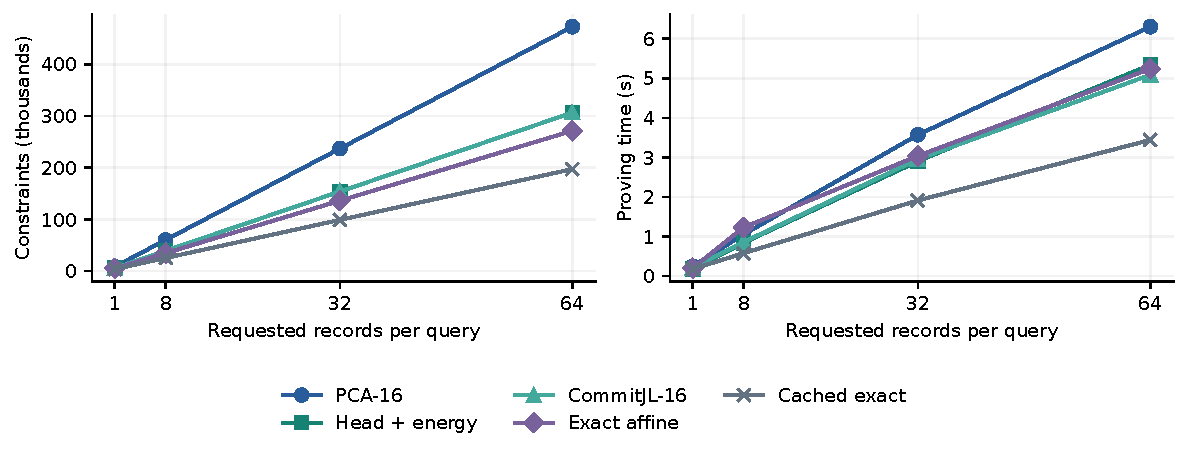
\includegraphics[width=0.93\textwidth]{paper_results/figures/scaling.pdf}
\caption{Actual query constraints and proving times as requested batch size grows under one fixed 64-row MNIST catalog, $k=5$. Preprocessing/setup are excluded. A full-catalog query has one possible subset.}
\label{fig:measured-scaling}
\end{figure*}

The principal ablation removes the JL tail while copying the same quantized head and energy (Table~\ref{tab:ablation-a}). Their fixed-center assignments and integer claimed costs are identical. The one-constraint difference in the new compiled contexts does not represent useful tail computation. Stage 1 does authenticate the tail and pays its derivation cost. On 48 capped corpus/$k$/start cells, head-only gives mean absolute aggregate-cost error 89.8338\%; adding energy lowers it to 0.004518\% without changing assignment. Replacing energy by the same tail norm gives 3.4380\% error. That same-tail no-energy control stores 15 rather than 16 statistics; equal-budget controls are also retained in the artifact.
\begin{table*}[tp]
\caption{Component attribution on the 48 capped corpus/$k$/start cells.}\label{tab:ablation-a}
\centering\small
\begin{adjustbox}{max width=\textwidth}
\begin{tabular}{@{}lrrrr@{}}
\toprule
Representation & Statistics/row & ARI vs. floating & Agreement (\%) & Mean absolute cost error (\%) \\
\midrule
Head only & $h$ & 0.99874 & 99.960 & 89.833826 \\
Head + energy & $h+1$ & 0.99874 & 99.960 & 0.004518 \\
Head + JL (no energy) & $15$ & 0.99589 & 99.841 & 3.437994 \\
CommitJL-16 & $16$ & 0.99874 & 99.960 & 0.004518 \\
PCA-16 & $16$ & 0.89294 & 95.502 & 74.443177 \\
\bottomrule
\end{tabular}
\end{adjustbox}
\par\vspace{3pt}\begin{minipage}{0.98\textwidth}\footnotesize Maps are first averaged within a start. Cost error is the absolute relative error of each cell's aggregate nearest-center cost, then averaged; it is not a signed bias or a per-point mean. The no-energy control keeps the same head and tail as CommitJL-16, so it stores 15 statistics. Its tail norm approximates residual energy; it is not added to an exact energy term. Equal-budget no-energy controls are also retained in the artifact. PCA error concerns use of projected cost as an original-cost proxy.\end{minipage}
\end{table*}


Increasing $k$ raises the protected rank and reduces the available tail budget. Native $k=2,20,50$ controls retain high agreement, but a rank-49 head plus energy cannot fit in 16 or 32 values. These budgets are explicitly excluded rather than silently truncating the protected span. Input and basis precision also matter: across the tested center counts, 8/8 scale bits give 99.3229\% floating-Full agreement and 0.580317\% mean absolute cost error, versus 99.9649\%/0.003861\% at 12/12 and 99.9953\%/0.000181\% at 16/16. These are native fidelity sweeps, not proof-time measurements at each precision.
\begin{table*}[tp]
\caption{Native protected-head sensitivity beyond five and ten centers.}\label{tab:centers}
\centering\small
\begin{adjustbox}{max width=\textwidth}
\begin{tabular}{@{}lrrrr@{}}
\toprule
Corpus & $k$ & Head/E statistics & ARI vs. quantized Full & Agreement (\%) \\
\midrule
Gaussian-hard & 2 & 2 & 1.00000 & 100.000 \\
Gaussian-hard & 20 & 20 & 0.99952 & 99.958 \\
Gaussian-hard & 50 & 50 & 0.99938 & 99.917 \\
MNIST & 2 & 2 & 1.00000 & 100.000 \\
MNIST & 20 & 20 & 0.99884 & 99.950 \\
MNIST & 50 & 50 & 0.99890 & 99.950 \\
\bottomrule
\end{tabular}
\end{adjustbox}
\par\vspace{3pt}\begin{minipage}{0.98\textwidth}\footnotesize Three starts per cell at input/basis scale bits 12. The head rank determines the minimum budget. At $k=50$, rank 49 plus energy requires 50 values; a 16- or 32-value head/tail representation is infeasible. No high-$k$ proof-time claim is inferred from these native checks.\end{minipage}
\end{table*}

\begin{table*}[tp]
\caption{Separate input and basis precision sensitivity for the protected representation.}\label{tab:precision}
\centering\small
\begin{adjustbox}{max width=\textwidth}
\begin{tabular}{@{}lrrr@{}}
\toprule
Input scale bits & Basis scale bits & Agreement vs. floating (\%) & Mean absolute cost error (\%) \\
\midrule
8 & 8 & 99.3229 & 0.580317 \\
8 & 12 & 99.4651 & 0.069845 \\
8 & 16 & 99.4566 & 0.067671 \\
12 & 8 & 99.7386 & 0.508827 \\
12 & 12 & 99.9649 & 0.003861 \\
12 & 16 & 99.9681 & 0.001427 \\
16 & 8 & 99.7716 & 0.508550 \\
16 & 12 & 99.9872 & 0.002856 \\
16 & 16 & 99.9953 & 0.000181 \\
\bottomrule
\end{tabular}
\end{adjustbox}
\par\vspace{3pt}\begin{minipage}{0.98\textwidth}\footnotesize Means over all tested native center-count cells: the 48 primary cells and 18 additional Gaussian-hard/MNIST cells at $k=2,20,50$. These native sweeps do not benchmark proof time or establish a minimum safe circuit bit width.\end{minipage}
\end{table*}


Plain sparse-map controls at one, two and four nonzeros per input column do not show a consistent fidelity improvement with density. This is why the fixed-center gain is attributed to the head/energy construction rather than a superior random matrix. The full density and normalized Rademacher controls, separate input/basis settings and model/compression/downstream times remain available as unrounded CSVs.

\subsection{Discussion}\label{sec:discussion}
\subsubsection{Useful regime and preprocessing cost}
The strongest current result is a compact, numerically accurate fixed-center query relation with lower measured proving cost than the tested PCA relation. The head+energy identity explains the quality, and the no-JL control identifies the source of the query savings. This is more specific than a claim that sparse random projections generally improve clustering or that dimension reduction always improves native runtime.

The completed implementation now binds the original catalog, fixed-point statistic derivation, ranges and authenticated subset indices under pinned roots/model/keys. A useful amortization experiment still needs genuinely different queries: unchanged records, centers and subset can reuse a previous answer or proof. The measured four-subset workload meets that distinction but is too small to establish a full-corpus crossover. Exact affine and cached-answer proofs are now available; cached exact answers are the stronger comparator when only nearest-center indices and minimum costs are required. The optional tail instead serves pair geometry, where its lower magnitude error is accompanied by weaker neighbor recall and greater authentication cost.

\subsubsection{Validity, security, and privacy limits}
Only one four-CPU, 7.76\,GiB host is represented in the new proof control. Three repeated timings per query, three primary native starts and five full-cached starts limit uncertainty estimates. There is no cross-dataset generalization interval or multiplicity-adjusted superiority claim. Largest proof catalogs contain 64 held-out records; full-cached native runs do not establish full-corpus proof feasibility. Actual proofs, native references, archived compilation-only rows and reconstructed workloads remain distinct.

Groth16 setup is circuit-specific. Because centers are constants, changing them can require a new representation, circuit and setup. Public costs, pair distances, centers/model, scales and query indices may reveal information; zero knowledge does not supply differential privacy or unlimited-query output privacy. The original owner root and setup/model manifest must be obtained authentically. The conditional single-stage theorem in Section~\ref{sec:theory} remains a specification-level result for plain sparse projection, separate from the completed approved-model integer binding. Its challenge-distribution premises are not supplied automatically by a successful proof. No fairness, distributed-beacon or unbounded grinding-resistance conclusion is inferred from the experiments.

\subsubsection{Reproducibility}
The artifact contains raw CSVs, per-case integer instances, verification outcomes, logs, resource records, source snapshots, dataset hashes and hash-verified receipts. Generated tables and figures remain under \texttt{paper\_results/}; its manifest distinguishes the completed Poseidon2 cohort from archived MiMC/order/margin studies. From the repository root, \path{code/analysis/revise_paper_results.py} and \path{code/analysis/export_targeted_paper_tables.py} regenerate numerical exports without rewriting the authored manuscript. The final review bundle is \path{code/results/final_paper_review_1792295389}. Full raw arrays and proof artifacts are preserved separately on the server; public exports exclude records, salts, assignments, caches and proving keys. Archived ordering/margin exports remain under \path{code/results/server_study_data_20261007}. Repository publication and persistent identifiers remain author-supplied metadata.
